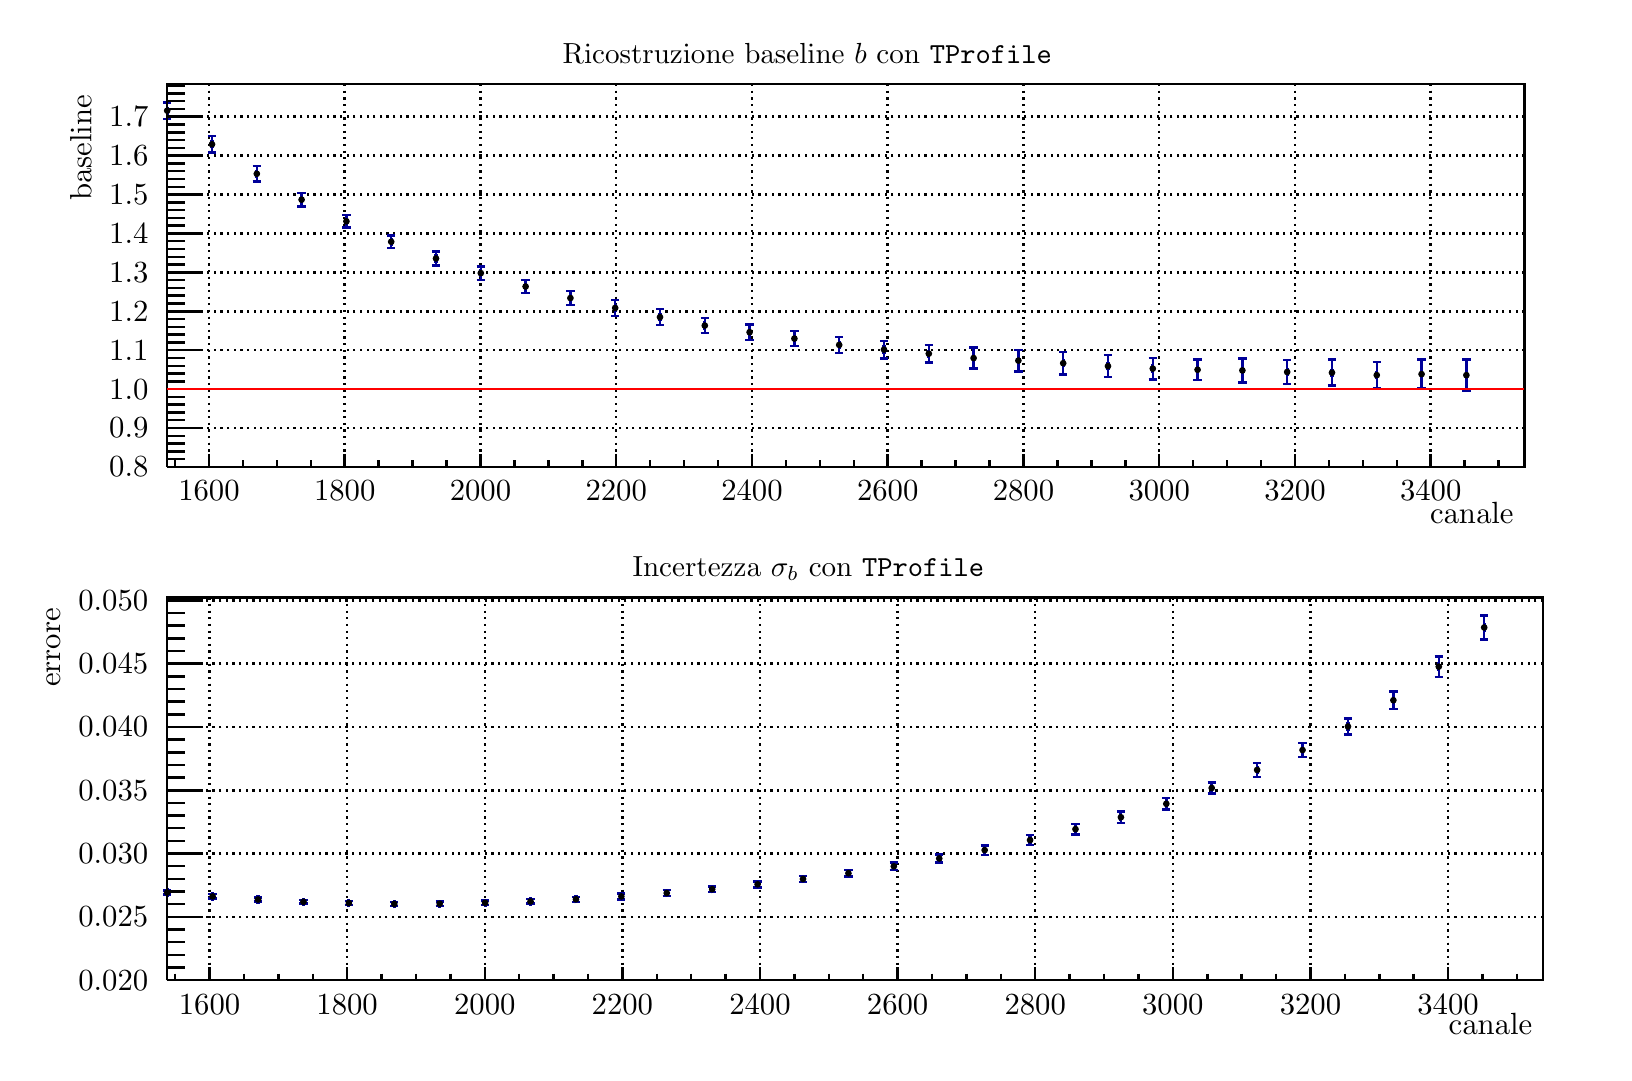
\begin{tikzpicture}
\pgfdeclareplotmark{cross} {
\pgfpathmoveto{\pgfpoint{-0.3\pgfplotmarksize}{\pgfplotmarksize}}
\pgfpathlineto{\pgfpoint{+0.3\pgfplotmarksize}{\pgfplotmarksize}}
\pgfpathlineto{\pgfpoint{+0.3\pgfplotmarksize}{0.3\pgfplotmarksize}}
\pgfpathlineto{\pgfpoint{+1\pgfplotmarksize}{0.3\pgfplotmarksize}}
\pgfpathlineto{\pgfpoint{+1\pgfplotmarksize}{-0.3\pgfplotmarksize}}
\pgfpathlineto{\pgfpoint{+0.3\pgfplotmarksize}{-0.3\pgfplotmarksize}}
\pgfpathlineto{\pgfpoint{+0.3\pgfplotmarksize}{-1.\pgfplotmarksize}}
\pgfpathlineto{\pgfpoint{-0.3\pgfplotmarksize}{-1.\pgfplotmarksize}}
\pgfpathlineto{\pgfpoint{-0.3\pgfplotmarksize}{-0.3\pgfplotmarksize}}
\pgfpathlineto{\pgfpoint{-1.\pgfplotmarksize}{-0.3\pgfplotmarksize}}
\pgfpathlineto{\pgfpoint{-1.\pgfplotmarksize}{0.3\pgfplotmarksize}}
\pgfpathlineto{\pgfpoint{-0.3\pgfplotmarksize}{0.3\pgfplotmarksize}}
\pgfpathclose
\pgfusepathqstroke
}
\pgfdeclareplotmark{cross*} {
\pgfpathmoveto{\pgfpoint{-0.3\pgfplotmarksize}{\pgfplotmarksize}}
\pgfpathlineto{\pgfpoint{+0.3\pgfplotmarksize}{\pgfplotmarksize}}
\pgfpathlineto{\pgfpoint{+0.3\pgfplotmarksize}{0.3\pgfplotmarksize}}
\pgfpathlineto{\pgfpoint{+1\pgfplotmarksize}{0.3\pgfplotmarksize}}
\pgfpathlineto{\pgfpoint{+1\pgfplotmarksize}{-0.3\pgfplotmarksize}}
\pgfpathlineto{\pgfpoint{+0.3\pgfplotmarksize}{-0.3\pgfplotmarksize}}
\pgfpathlineto{\pgfpoint{+0.3\pgfplotmarksize}{-1.\pgfplotmarksize}}
\pgfpathlineto{\pgfpoint{-0.3\pgfplotmarksize}{-1.\pgfplotmarksize}}
\pgfpathlineto{\pgfpoint{-0.3\pgfplotmarksize}{-0.3\pgfplotmarksize}}
\pgfpathlineto{\pgfpoint{-1.\pgfplotmarksize}{-0.3\pgfplotmarksize}}
\pgfpathlineto{\pgfpoint{-1.\pgfplotmarksize}{0.3\pgfplotmarksize}}
\pgfpathlineto{\pgfpoint{-0.3\pgfplotmarksize}{0.3\pgfplotmarksize}}
\pgfpathclose
\pgfusepathqfillstroke
}
\pgfdeclareplotmark{newstar} {
\pgfpathmoveto{\pgfqpoint{0pt}{\pgfplotmarksize}}
\pgfpathlineto{\pgfqpointpolar{44}{0.5\pgfplotmarksize}}
\pgfpathlineto{\pgfqpointpolar{18}{\pgfplotmarksize}}
\pgfpathlineto{\pgfqpointpolar{-20}{0.5\pgfplotmarksize}}
\pgfpathlineto{\pgfqpointpolar{-54}{\pgfplotmarksize}}
\pgfpathlineto{\pgfqpointpolar{-90}{0.5\pgfplotmarksize}}
\pgfpathlineto{\pgfqpointpolar{234}{\pgfplotmarksize}}
\pgfpathlineto{\pgfqpointpolar{198}{0.5\pgfplotmarksize}}
\pgfpathlineto{\pgfqpointpolar{162}{\pgfplotmarksize}}
\pgfpathlineto{\pgfqpointpolar{134}{0.5\pgfplotmarksize}}
\pgfpathclose
\pgfusepathqstroke
}
\pgfdeclareplotmark{newstar*} {
\pgfpathmoveto{\pgfqpoint{0pt}{\pgfplotmarksize}}
\pgfpathlineto{\pgfqpointpolar{44}{0.5\pgfplotmarksize}}
\pgfpathlineto{\pgfqpointpolar{18}{\pgfplotmarksize}}
\pgfpathlineto{\pgfqpointpolar{-20}{0.5\pgfplotmarksize}}
\pgfpathlineto{\pgfqpointpolar{-54}{\pgfplotmarksize}}
\pgfpathlineto{\pgfqpointpolar{-90}{0.5\pgfplotmarksize}}
\pgfpathlineto{\pgfqpointpolar{234}{\pgfplotmarksize}}
\pgfpathlineto{\pgfqpointpolar{198}{0.5\pgfplotmarksize}}
\pgfpathlineto{\pgfqpointpolar{162}{\pgfplotmarksize}}
\pgfpathlineto{\pgfqpointpolar{134}{0.5\pgfplotmarksize}}
\pgfpathclose
\pgfusepathqfillstroke
}
\definecolor{c}{rgb}{1,1,1};
\draw [color=c, fill=c] (0,0) rectangle (20,13.0092);
\draw [color=c, fill=c] (0.197109,6.64915) rectangle (19.6189,12.9041);
\draw [color=c, fill=c] (1.76084,7.43758) rectangle (19.0013,12.2996);
\definecolor{c}{rgb}{0,0,0};
\draw [c,line width=0.9] (1.76084,7.43758) -- (1.76084,12.2996) -- (19.0013,12.2996) -- (19.0013,7.43758) -- (1.76084,7.43758);
\definecolor{c}{rgb}{1,1,1};
\draw [color=c, fill=c] (1.76084,7.43758) rectangle (19.0013,12.2996);
\definecolor{c}{rgb}{0,0,0};
\draw [c,line width=0.9] (1.76084,7.43758) -- (1.76084,12.2996) -- (19.0013,12.2996) -- (19.0013,7.43758) -- (1.76084,7.43758);
\draw [c,line width=0.9] (1.76084,7.43758) -- (19.0013,7.43758);
\draw [c,dash pattern=on 0.80pt off 1.60pt ,line width=0.9] (2.2953,12.2996) -- (2.2953,7.43758);
\draw [c,dash pattern=on 0.80pt off 1.60pt ,line width=0.9] (4.01934,12.2996) -- (4.01934,7.43758);
\draw [c,dash pattern=on 0.80pt off 1.60pt ,line width=0.9] (5.74339,12.2996) -- (5.74339,7.43758);
\draw [c,dash pattern=on 0.80pt off 1.60pt ,line width=0.9] (7.46744,12.2996) -- (7.46744,7.43758);
\draw [c,dash pattern=on 0.80pt off 1.60pt ,line width=0.9] (9.19148,12.2996) -- (9.19148,7.43758);
\draw [c,dash pattern=on 0.80pt off 1.60pt ,line width=0.9] (10.9155,12.2996) -- (10.9155,7.43758);
\draw [c,dash pattern=on 0.80pt off 1.60pt ,line width=0.9] (12.6396,12.2996) -- (12.6396,7.43758);
\draw [c,dash pattern=on 0.80pt off 1.60pt ,line width=0.9] (14.3636,12.2996) -- (14.3636,7.43758);
\draw [c,dash pattern=on 0.80pt off 1.60pt ,line width=0.9] (16.0877,12.2996) -- (16.0877,7.43758);
\draw [c,dash pattern=on 0.80pt off 1.60pt ,line width=0.9] (17.8117,12.2996) -- (17.8117,7.43758);
\draw [c,dash pattern=on 0.80pt off 1.60pt ,line width=0.9] (2.2953,12.2996) -- (2.2953,7.43758);
\draw [c,dash pattern=on 0.80pt off 1.60pt ,line width=0.9] (17.8117,12.2996) -- (17.8117,7.43758);
\draw [c,line width=0.9] (1.76084,7.43758) -- (1.76084,12.2996);
\draw [c,dash pattern=on 0.80pt off 1.60pt ,line width=0.9] (19.0013,7.43758) -- (1.76084,7.43758);
\draw [c,dash pattern=on 0.80pt off 1.60pt ,line width=0.9] (19.0013,7.93174) -- (1.76084,7.93174);
\draw [c,dash pattern=on 0.80pt off 1.60pt ,line width=0.9] (19.0013,8.4259) -- (1.76084,8.4259);
\draw [c,dash pattern=on 0.80pt off 1.60pt ,line width=0.9] (19.0013,8.92006) -- (1.76084,8.92006);
\draw [c,dash pattern=on 0.80pt off 1.60pt ,line width=0.9] (19.0013,9.41422) -- (1.76084,9.41422);
\draw [c,dash pattern=on 0.80pt off 1.60pt ,line width=0.9] (19.0013,9.90838) -- (1.76084,9.90838);
\draw [c,dash pattern=on 0.80pt off 1.60pt ,line width=0.9] (19.0013,10.4025) -- (1.76084,10.4025);
\draw [c,dash pattern=on 0.80pt off 1.60pt ,line width=0.9] (19.0013,10.8967) -- (1.76084,10.8967);
\draw [c,dash pattern=on 0.80pt off 1.60pt ,line width=0.9] (19.0013,11.3909) -- (1.76084,11.3909);
\draw [c,dash pattern=on 0.80pt off 1.60pt ,line width=0.9] (19.0013,11.885) -- (1.76084,11.885);
\draw [c,dash pattern=on 0.80pt off 1.60pt ,line width=0.9] (19.0013,11.885) -- (1.76084,11.885);
\definecolor{c}{rgb}{0,0,0.6};
\draw [c,line width=0.9] (1.76515,11.8559) -- (1.76515,11.962);
\draw [c,line width=0.9] (1.76515,11.962) -- (1.76515,12.0681);
\draw [c,line width=0.9] (1.76084,11.962) -- (1.76515,11.962);
\draw [c,line width=0.9] (1.76515,11.962) -- (1.76946,11.962);
\draw [c,line width=0.9] (1.71259,11.8559) -- (1.81771,11.8559);
\draw [c,line width=0.9] (1.71259,12.0681) -- (1.81771,12.0681);
\draw [c,line width=0.9] (1.76084,11.9094) -- (1.76084,12.0146);
\draw [c,line width=0.9] (1.76946,11.9094) -- (1.76946,12.0146);
\definecolor{c}{rgb}{0,0,0};
\foreach \P in {(1.76515,11.962)}{\draw[mark options={color=c,fill=c},mark size=2.402402pt,mark=*,mark size=1pt] plot coordinates {\P};}
\definecolor{c}{rgb}{0,0,0.6};
\draw [c,line width=0.9] (2.33409,11.4287) -- (2.33409,11.5349);
\draw [c,line width=0.9] (2.33409,11.5349) -- (2.33409,11.6411);
\draw [c,line width=0.9] (2.32978,11.5349) -- (2.33409,11.5349);
\draw [c,line width=0.9] (2.33409,11.5349) -- (2.3384,11.5349);
\draw [c,line width=0.9] (2.28152,11.4287) -- (2.38665,11.4287);
\draw [c,line width=0.9] (2.28152,11.6411) -- (2.38665,11.6411);
\draw [c,line width=0.9] (2.32978,11.4824) -- (2.32978,11.5875);
\draw [c,line width=0.9] (2.3384,11.4824) -- (2.3384,11.5875);
\definecolor{c}{rgb}{0,0,0};
\foreach \P in {(2.33409,11.5349)}{\draw[mark options={color=c,fill=c},mark size=2.402402pt,mark=*,mark size=1pt] plot coordinates {\P};}
\definecolor{c}{rgb}{0,0,0.6};
\draw [c,line width=0.9] (2.90302,11.0641) -- (2.90302,11.1606);
\draw [c,line width=0.9] (2.90302,11.1606) -- (2.90302,11.257);
\draw [c,line width=0.9] (2.89871,11.1606) -- (2.90302,11.1606);
\draw [c,line width=0.9] (2.90302,11.1606) -- (2.90733,11.1606);
\draw [c,line width=0.9] (2.85046,11.0641) -- (2.95558,11.0641);
\draw [c,line width=0.9] (2.85046,11.257) -- (2.95558,11.257);
\draw [c,line width=0.9] (2.89871,11.108) -- (2.89871,11.2131);
\draw [c,line width=0.9] (2.90733,11.108) -- (2.90733,11.2131);
\definecolor{c}{rgb}{0,0,0};
\foreach \P in {(2.90302,11.1606)}{\draw[mark options={color=c,fill=c},mark size=2.402402pt,mark=*,mark size=1pt] plot coordinates {\P};}
\definecolor{c}{rgb}{0,0,0.6};
\draw [c,line width=0.9] (3.47196,10.7466) -- (3.47196,10.8316);
\draw [c,line width=0.9] (3.47196,10.8316) -- (3.47196,10.9167);
\draw [c,line width=0.9] (3.46765,10.8316) -- (3.47196,10.8316);
\draw [c,line width=0.9] (3.47196,10.8316) -- (3.47627,10.8316);
\draw [c,line width=0.9] (3.4194,10.7466) -- (3.52452,10.7466);
\draw [c,line width=0.9] (3.4194,10.9167) -- (3.52452,10.9167);
\draw [c,line width=0.9] (3.46765,10.7791) -- (3.46765,10.8842);
\draw [c,line width=0.9] (3.47627,10.7791) -- (3.47627,10.8842);
\definecolor{c}{rgb}{0,0,0};
\foreach \P in {(3.47196,10.8316)}{\draw[mark options={color=c,fill=c},mark size=2.402402pt,mark=*,mark size=1pt] plot coordinates {\P};}
\definecolor{c}{rgb}{0,0,0.6};
\draw [c,line width=0.9] (4.04089,10.4778) -- (4.04089,10.5565);
\draw [c,line width=0.9] (4.04089,10.5565) -- (4.04089,10.6353);
\draw [c,line width=0.9] (4.03658,10.5565) -- (4.04089,10.5565);
\draw [c,line width=0.9] (4.04089,10.5565) -- (4.0452,10.5565);
\draw [c,line width=0.9] (3.98833,10.4778) -- (4.09346,10.4778);
\draw [c,line width=0.9] (3.98833,10.6353) -- (4.09346,10.6353);
\draw [c,line width=0.9] (4.03658,10.504) -- (4.03658,10.6091);
\draw [c,line width=0.9] (4.0452,10.504) -- (4.0452,10.6091);
\definecolor{c}{rgb}{0,0,0};
\foreach \P in {(4.04089,10.5565)}{\draw[mark options={color=c,fill=c},mark size=2.402402pt,mark=*,mark size=1pt] plot coordinates {\P};}
\definecolor{c}{rgb}{0,0,0.6};
\draw [c,line width=0.9] (4.60983,10.2184) -- (4.60983,10.297);
\draw [c,line width=0.9] (4.60983,10.297) -- (4.60983,10.3755);
\draw [c,line width=0.9] (4.60552,10.297) -- (4.60983,10.297);
\draw [c,line width=0.9] (4.60983,10.297) -- (4.61414,10.297);
\draw [c,line width=0.9] (4.55727,10.2184) -- (4.66239,10.2184);
\draw [c,line width=0.9] (4.55727,10.3755) -- (4.66239,10.3755);
\draw [c,line width=0.9] (4.60552,10.2444) -- (4.60552,10.3495);
\draw [c,line width=0.9] (4.61414,10.2444) -- (4.61414,10.3495);
\definecolor{c}{rgb}{0,0,0};
\foreach \P in {(4.60983,10.297)}{\draw[mark options={color=c,fill=c},mark size=2.402402pt,mark=*,mark size=1pt] plot coordinates {\P};}
\definecolor{c}{rgb}{0,0,0.6};
\draw [c,line width=0.9] (5.17876,9.99563) -- (5.17876,10.0852);
\draw [c,line width=0.9] (5.17876,10.0852) -- (5.17876,10.1748);
\draw [c,line width=0.9] (5.17445,10.0852) -- (5.17876,10.0852);
\draw [c,line width=0.9] (5.17876,10.0852) -- (5.18307,10.0852);
\draw [c,line width=0.9] (5.1262,9.99563) -- (5.23133,9.99563);
\draw [c,line width=0.9] (5.1262,10.1748) -- (5.23133,10.1748);
\draw [c,line width=0.9] (5.17445,10.0326) -- (5.17445,10.1378);
\draw [c,line width=0.9] (5.18307,10.0326) -- (5.18307,10.1378);
\definecolor{c}{rgb}{0,0,0};
\foreach \P in {(5.17876,10.0852)}{\draw[mark options={color=c,fill=c},mark size=2.402402pt,mark=*,mark size=1pt] plot coordinates {\P};}
\definecolor{c}{rgb}{0,0,0.6};
\draw [c,line width=0.9] (5.7477,9.81474) -- (5.7477,9.89912);
\draw [c,line width=0.9] (5.7477,9.89912) -- (5.7477,9.9835);
\draw [c,line width=0.9] (5.74339,9.89912) -- (5.7477,9.89912);
\draw [c,line width=0.9] (5.7477,9.89912) -- (5.75201,9.89912);
\draw [c,line width=0.9] (5.69514,9.81474) -- (5.80026,9.81474);
\draw [c,line width=0.9] (5.69514,9.9835) -- (5.80026,9.9835);
\draw [c,line width=0.9] (5.74339,9.84656) -- (5.74339,9.95168);
\draw [c,line width=0.9] (5.75201,9.84656) -- (5.75201,9.95168);
\definecolor{c}{rgb}{0,0,0};
\foreach \P in {(5.7477,9.89912)}{\draw[mark options={color=c,fill=c},mark size=2.402402pt,mark=*,mark size=1pt] plot coordinates {\P};}
\definecolor{c}{rgb}{0,0,0.6};
\draw [c,line width=0.9] (6.31664,9.64435) -- (6.31664,9.72887);
\draw [c,line width=0.9] (6.31664,9.72887) -- (6.31664,9.81339);
\draw [c,line width=0.9] (6.31233,9.72887) -- (6.31664,9.72887);
\draw [c,line width=0.9] (6.31664,9.72887) -- (6.32095,9.72887);
\draw [c,line width=0.9] (6.26407,9.64435) -- (6.3692,9.64435);
\draw [c,line width=0.9] (6.26407,9.81339) -- (6.3692,9.81339);
\draw [c,line width=0.9] (6.31233,9.67631) -- (6.31233,9.78143);
\draw [c,line width=0.9] (6.32095,9.67631) -- (6.32095,9.78143);
\definecolor{c}{rgb}{0,0,0};
\foreach \P in {(6.31664,9.72887)}{\draw[mark options={color=c,fill=c},mark size=2.402402pt,mark=*,mark size=1pt] plot coordinates {\P};}
\definecolor{c}{rgb}{0,0,0.6};
\draw [c,line width=0.9] (6.88557,9.49105) -- (6.88557,9.58247);
\draw [c,line width=0.9] (6.88557,9.58247) -- (6.88557,9.6739);
\draw [c,line width=0.9] (6.88126,9.58247) -- (6.88557,9.58247);
\draw [c,line width=0.9] (6.88557,9.58247) -- (6.88988,9.58247);
\draw [c,line width=0.9] (6.83301,9.49105) -- (6.93813,9.49105);
\draw [c,line width=0.9] (6.83301,9.6739) -- (6.93813,9.6739);
\draw [c,line width=0.9] (6.88126,9.52991) -- (6.88126,9.63504);
\draw [c,line width=0.9] (6.88988,9.52991) -- (6.88988,9.63504);
\definecolor{c}{rgb}{0,0,0};
\foreach \P in {(6.88557,9.58247)}{\draw[mark options={color=c,fill=c},mark size=2.402402pt,mark=*,mark size=1pt] plot coordinates {\P};}
\definecolor{c}{rgb}{0,0,0.6};
\draw [c,line width=0.9] (7.45451,9.35429) -- (7.45451,9.4567);
\draw [c,line width=0.9] (7.45451,9.4567) -- (7.45451,9.5591);
\draw [c,line width=0.9] (7.4502,9.4567) -- (7.45451,9.4567);
\draw [c,line width=0.9] (7.45451,9.4567) -- (7.45882,9.4567);
\draw [c,line width=0.9] (7.40194,9.35429) -- (7.50707,9.35429);
\draw [c,line width=0.9] (7.40194,9.5591) -- (7.50707,9.5591);
\draw [c,line width=0.9] (7.4502,9.40414) -- (7.4502,9.50926);
\draw [c,line width=0.9] (7.45882,9.40414) -- (7.45882,9.50926);
\definecolor{c}{rgb}{0,0,0};
\foreach \P in {(7.45451,9.4567)}{\draw[mark options={color=c,fill=c},mark size=2.402402pt,mark=*,mark size=1pt] plot coordinates {\P};}
\definecolor{c}{rgb}{0,0,0.6};
\draw [c,line width=0.9] (8.02344,9.23709) -- (8.02344,9.34039);
\draw [c,line width=0.9] (8.02344,9.34039) -- (8.02344,9.44369);
\draw [c,line width=0.9] (8.01913,9.34039) -- (8.02344,9.34039);
\draw [c,line width=0.9] (8.02344,9.34039) -- (8.02775,9.34039);
\draw [c,line width=0.9] (7.97088,9.23709) -- (8.076,9.23709);
\draw [c,line width=0.9] (7.97088,9.44369) -- (8.076,9.44369);
\draw [c,line width=0.9] (8.01913,9.28783) -- (8.01913,9.39295);
\draw [c,line width=0.9] (8.02775,9.28783) -- (8.02775,9.39295);
\definecolor{c}{rgb}{0,0,0};
\foreach \P in {(8.02344,9.34039)}{\draw[mark options={color=c,fill=c},mark size=2.402402pt,mark=*,mark size=1pt] plot coordinates {\P};}
\definecolor{c}{rgb}{0,0,0.6};
\draw [c,line width=0.9] (8.59238,9.13913) -- (8.59238,9.23286);
\draw [c,line width=0.9] (8.59238,9.23286) -- (8.59238,9.3266);
\draw [c,line width=0.9] (8.58807,9.23286) -- (8.59238,9.23286);
\draw [c,line width=0.9] (8.59238,9.23286) -- (8.59669,9.23286);
\draw [c,line width=0.9] (8.53982,9.13913) -- (8.64494,9.13913);
\draw [c,line width=0.9] (8.53982,9.3266) -- (8.64494,9.3266);
\draw [c,line width=0.9] (8.58807,9.1803) -- (8.58807,9.28543);
\draw [c,line width=0.9] (8.59669,9.1803) -- (8.59669,9.28543);
\definecolor{c}{rgb}{0,0,0};
\foreach \P in {(8.59238,9.23286)}{\draw[mark options={color=c,fill=c},mark size=2.402402pt,mark=*,mark size=1pt] plot coordinates {\P};}
\definecolor{c}{rgb}{0,0,0.6};
\draw [c,line width=0.9] (9.16131,9.05208) -- (9.16131,9.14867);
\draw [c,line width=0.9] (9.16131,9.14867) -- (9.16131,9.24526);
\draw [c,line width=0.9] (9.157,9.14867) -- (9.16131,9.14867);
\draw [c,line width=0.9] (9.16131,9.14867) -- (9.16562,9.14867);
\draw [c,line width=0.9] (9.10875,9.05208) -- (9.21388,9.05208);
\draw [c,line width=0.9] (9.10875,9.24526) -- (9.21388,9.24526);
\draw [c,line width=0.9] (9.157,9.09611) -- (9.157,9.20123);
\draw [c,line width=0.9] (9.16562,9.09611) -- (9.16562,9.20123);
\definecolor{c}{rgb}{0,0,0};
\foreach \P in {(9.16131,9.14867)}{\draw[mark options={color=c,fill=c},mark size=2.402402pt,mark=*,mark size=1pt] plot coordinates {\P};}
\definecolor{c}{rgb}{0,0,0.6};
\draw [c,line width=0.9] (9.73025,8.97208) -- (9.73025,9.06787);
\draw [c,line width=0.9] (9.73025,9.06787) -- (9.73025,9.16365);
\draw [c,line width=0.9] (9.72594,9.06787) -- (9.73025,9.06787);
\draw [c,line width=0.9] (9.73025,9.06787) -- (9.73456,9.06787);
\draw [c,line width=0.9] (9.67769,8.97208) -- (9.78281,8.97208);
\draw [c,line width=0.9] (9.67769,9.16365) -- (9.78281,9.16365);
\draw [c,line width=0.9] (9.72594,9.0153) -- (9.72594,9.12043);
\draw [c,line width=0.9] (9.73456,9.0153) -- (9.73456,9.12043);
\definecolor{c}{rgb}{0,0,0};
\foreach \P in {(9.73025,9.06787)}{\draw[mark options={color=c,fill=c},mark size=2.402402pt,mark=*,mark size=1pt] plot coordinates {\P};}
\definecolor{c}{rgb}{0,0,0.6};
\draw [c,line width=0.9] (10.2992,8.88708) -- (10.2992,8.98708);
\draw [c,line width=0.9] (10.2992,8.98708) -- (10.2992,9.08707);
\draw [c,line width=0.9] (10.2949,8.98708) -- (10.2992,8.98708);
\draw [c,line width=0.9] (10.2992,8.98708) -- (10.3035,8.98708);
\draw [c,line width=0.9] (10.2466,8.88708) -- (10.3517,8.88708);
\draw [c,line width=0.9] (10.2466,9.08707) -- (10.3517,9.08707);
\draw [c,line width=0.9] (10.2949,8.93452) -- (10.2949,9.03964);
\draw [c,line width=0.9] (10.3035,8.93452) -- (10.3035,9.03964);
\definecolor{c}{rgb}{0,0,0};
\foreach \P in {(10.2992,8.98708)}{\draw[mark options={color=c,fill=c},mark size=2.402402pt,mark=*,mark size=1pt] plot coordinates {\P};}
\definecolor{c}{rgb}{0,0,0.6};
\draw [c,line width=0.9] (10.8681,8.81572) -- (10.8681,8.92722);
\draw [c,line width=0.9] (10.8681,8.92722) -- (10.8681,9.03872);
\draw [c,line width=0.9] (10.8638,8.92722) -- (10.8681,8.92722);
\draw [c,line width=0.9] (10.8681,8.92722) -- (10.8724,8.92722);
\draw [c,line width=0.9] (10.8156,8.81572) -- (10.9207,8.81572);
\draw [c,line width=0.9] (10.8156,9.03872) -- (10.9207,9.03872);
\draw [c,line width=0.9] (10.8638,8.87466) -- (10.8638,8.97978);
\draw [c,line width=0.9] (10.8724,8.87466) -- (10.8724,8.97978);
\definecolor{c}{rgb}{0,0,0};
\foreach \P in {(10.8681,8.92722)}{\draw[mark options={color=c,fill=c},mark size=2.402402pt,mark=*,mark size=1pt] plot coordinates {\P};}
\definecolor{c}{rgb}{0,0,0.6};
\draw [c,line width=0.9] (11.4371,8.76513) -- (11.4371,8.87623);
\draw [c,line width=0.9] (11.4371,8.87623) -- (11.4371,8.98733);
\draw [c,line width=0.9] (11.4327,8.87623) -- (11.4371,8.87623);
\draw [c,line width=0.9] (11.4371,8.87623) -- (11.4414,8.87623);
\draw [c,line width=0.9] (11.3845,8.76513) -- (11.4896,8.76513);
\draw [c,line width=0.9] (11.3845,8.98733) -- (11.4896,8.98733);
\draw [c,line width=0.9] (11.4327,8.82367) -- (11.4327,8.92879);
\draw [c,line width=0.9] (11.4414,8.82367) -- (11.4414,8.92879);
\definecolor{c}{rgb}{0,0,0};
\foreach \P in {(11.4371,8.87623)}{\draw[mark options={color=c,fill=c},mark size=2.402402pt,mark=*,mark size=1pt] plot coordinates {\P};}
\definecolor{c}{rgb}{0,0,0.6};
\draw [c,line width=0.9] (12.006,8.68691) -- (12.006,8.82007);
\draw [c,line width=0.9] (12.006,8.82007) -- (12.006,8.95324);
\draw [c,line width=0.9] (12.0017,8.82007) -- (12.006,8.82007);
\draw [c,line width=0.9] (12.006,8.82007) -- (12.0103,8.82007);
\draw [c,line width=0.9] (11.9534,8.68691) -- (12.0586,8.68691);
\draw [c,line width=0.9] (11.9534,8.95324) -- (12.0586,8.95324);
\draw [c,line width=0.9] (12.0017,8.76751) -- (12.0017,8.87264);
\draw [c,line width=0.9] (12.0103,8.76751) -- (12.0103,8.87264);
\definecolor{c}{rgb}{0,0,0};
\foreach \P in {(12.006,8.82007)}{\draw[mark options={color=c,fill=c},mark size=2.402402pt,mark=*,mark size=1pt] plot coordinates {\P};}
\definecolor{c}{rgb}{0,0,0.6};
\draw [c,line width=0.9] (12.5749,8.65095) -- (12.5749,8.78791);
\draw [c,line width=0.9] (12.5749,8.78791) -- (12.5749,8.92487);
\draw [c,line width=0.9] (12.5706,8.78791) -- (12.5749,8.78791);
\draw [c,line width=0.9] (12.5749,8.78791) -- (12.5792,8.78791);
\draw [c,line width=0.9] (12.5224,8.65095) -- (12.6275,8.65095);
\draw [c,line width=0.9] (12.5224,8.92487) -- (12.6275,8.92487);
\draw [c,line width=0.9] (12.5706,8.73535) -- (12.5706,8.84047);
\draw [c,line width=0.9] (12.5792,8.73535) -- (12.5792,8.84047);
\definecolor{c}{rgb}{0,0,0};
\foreach \P in {(12.5749,8.78791)}{\draw[mark options={color=c,fill=c},mark size=2.402402pt,mark=*,mark size=1pt] plot coordinates {\P};}
\definecolor{c}{rgb}{0,0,0.6};
\draw [c,line width=0.9] (13.1439,8.61429) -- (13.1439,8.7547);
\draw [c,line width=0.9] (13.1439,8.7547) -- (13.1439,8.8951);
\draw [c,line width=0.9] (13.1396,8.7547) -- (13.1439,8.7547);
\draw [c,line width=0.9] (13.1439,8.7547) -- (13.1482,8.7547);
\draw [c,line width=0.9] (13.0913,8.61429) -- (13.1964,8.61429);
\draw [c,line width=0.9] (13.0913,8.8951) -- (13.1964,8.8951);
\draw [c,line width=0.9] (13.1396,8.70213) -- (13.1396,8.80726);
\draw [c,line width=0.9] (13.1482,8.70213) -- (13.1482,8.80726);
\definecolor{c}{rgb}{0,0,0};
\foreach \P in {(13.1439,8.7547)}{\draw[mark options={color=c,fill=c},mark size=2.402402pt,mark=*,mark size=1pt] plot coordinates {\P};}
\definecolor{c}{rgb}{0,0,0.6};
\draw [c,line width=0.9] (13.7128,8.57775) -- (13.7128,8.71784);
\draw [c,line width=0.9] (13.7128,8.71784) -- (13.7128,8.85792);
\draw [c,line width=0.9] (13.7085,8.71784) -- (13.7128,8.71784);
\draw [c,line width=0.9] (13.7128,8.71784) -- (13.7171,8.71784);
\draw [c,line width=0.9] (13.6602,8.57775) -- (13.7654,8.57775);
\draw [c,line width=0.9] (13.6602,8.85792) -- (13.7654,8.85792);
\draw [c,line width=0.9] (13.7085,8.66528) -- (13.7085,8.7704);
\draw [c,line width=0.9] (13.7171,8.66528) -- (13.7171,8.7704);
\definecolor{c}{rgb}{0,0,0};
\foreach \P in {(13.7128,8.71784)}{\draw[mark options={color=c,fill=c},mark size=2.402402pt,mark=*,mark size=1pt] plot coordinates {\P};}
\definecolor{c}{rgb}{0,0,0.6};
\draw [c,line width=0.9] (14.2817,8.54836) -- (14.2817,8.68595);
\draw [c,line width=0.9] (14.2817,8.68595) -- (14.2817,8.82354);
\draw [c,line width=0.9] (14.2774,8.68595) -- (14.2817,8.68595);
\draw [c,line width=0.9] (14.2817,8.68595) -- (14.286,8.68595);
\draw [c,line width=0.9] (14.2292,8.54836) -- (14.3343,8.54836);
\draw [c,line width=0.9] (14.2292,8.82354) -- (14.3343,8.82354);
\draw [c,line width=0.9] (14.2774,8.63339) -- (14.2774,8.73851);
\draw [c,line width=0.9] (14.286,8.63339) -- (14.286,8.73851);
\definecolor{c}{rgb}{0,0,0};
\foreach \P in {(14.2817,8.68595)}{\draw[mark options={color=c,fill=c},mark size=2.402402pt,mark=*,mark size=1pt] plot coordinates {\P};}
\definecolor{c}{rgb}{0,0,0.6};
\draw [c,line width=0.9] (14.8507,8.53843) -- (14.8507,8.67161);
\draw [c,line width=0.9] (14.8507,8.67161) -- (14.8507,8.80479);
\draw [c,line width=0.9] (14.8464,8.67161) -- (14.8507,8.67161);
\draw [c,line width=0.9] (14.8507,8.67161) -- (14.855,8.67161);
\draw [c,line width=0.9] (14.7981,8.53843) -- (14.9032,8.53843);
\draw [c,line width=0.9] (14.7981,8.80479) -- (14.9032,8.80479);
\draw [c,line width=0.9] (14.8464,8.61905) -- (14.8464,8.72417);
\draw [c,line width=0.9] (14.855,8.61905) -- (14.855,8.72417);
\definecolor{c}{rgb}{0,0,0};
\foreach \P in {(14.8507,8.67161)}{\draw[mark options={color=c,fill=c},mark size=2.402402pt,mark=*,mark size=1pt] plot coordinates {\P};}
\definecolor{c}{rgb}{0,0,0.6};
\draw [c,line width=0.9] (15.4196,8.50924) -- (15.4196,8.66328);
\draw [c,line width=0.9] (15.4196,8.66328) -- (15.4196,8.81732);
\draw [c,line width=0.9] (15.4153,8.66328) -- (15.4196,8.66328);
\draw [c,line width=0.9] (15.4196,8.66328) -- (15.4239,8.66328);
\draw [c,line width=0.9] (15.367,8.50924) -- (15.4722,8.50924);
\draw [c,line width=0.9] (15.367,8.81732) -- (15.4722,8.81732);
\draw [c,line width=0.9] (15.4153,8.61072) -- (15.4153,8.71585);
\draw [c,line width=0.9] (15.4239,8.61072) -- (15.4239,8.71585);
\definecolor{c}{rgb}{0,0,0};
\foreach \P in {(15.4196,8.66328)}{\draw[mark options={color=c,fill=c},mark size=2.402402pt,mark=*,mark size=1pt] plot coordinates {\P};}
\definecolor{c}{rgb}{0,0,0.6};
\draw [c,line width=0.9] (15.9885,8.49137) -- (15.9885,8.64307);
\draw [c,line width=0.9] (15.9885,8.64307) -- (15.9885,8.79476);
\draw [c,line width=0.9] (15.9842,8.64307) -- (15.9885,8.64307);
\draw [c,line width=0.9] (15.9885,8.64307) -- (15.9929,8.64307);
\draw [c,line width=0.9] (15.936,8.49137) -- (16.0411,8.49137);
\draw [c,line width=0.9] (15.936,8.79476) -- (16.0411,8.79476);
\draw [c,line width=0.9] (15.9842,8.5905) -- (15.9842,8.69563);
\draw [c,line width=0.9] (15.9929,8.5905) -- (15.9929,8.69563);
\definecolor{c}{rgb}{0,0,0};
\foreach \P in {(15.9885,8.64307)}{\draw[mark options={color=c,fill=c},mark size=2.402402pt,mark=*,mark size=1pt] plot coordinates {\P};}
\definecolor{c}{rgb}{0,0,0.6};
\draw [c,line width=0.9] (16.5575,8.46942) -- (16.5575,8.63446);
\draw [c,line width=0.9] (16.5575,8.63446) -- (16.5575,8.79949);
\draw [c,line width=0.9] (16.5532,8.63446) -- (16.5575,8.63446);
\draw [c,line width=0.9] (16.5575,8.63446) -- (16.5618,8.63446);
\draw [c,line width=0.9] (16.5049,8.46942) -- (16.61,8.46942);
\draw [c,line width=0.9] (16.5049,8.79949) -- (16.61,8.79949);
\draw [c,line width=0.9] (16.5532,8.58189) -- (16.5532,8.68702);
\draw [c,line width=0.9] (16.5618,8.58189) -- (16.5618,8.68702);
\definecolor{c}{rgb}{0,0,0};
\foreach \P in {(16.5575,8.63446)}{\draw[mark options={color=c,fill=c},mark size=2.402402pt,mark=*,mark size=1pt] plot coordinates {\P};}
\definecolor{c}{rgb}{0,0,0.6};
\draw [c,line width=0.9] (17.1264,8.43704) -- (17.1264,8.60359);
\draw [c,line width=0.9] (17.1264,8.60359) -- (17.1264,8.77014);
\draw [c,line width=0.9] (17.1221,8.60359) -- (17.1264,8.60359);
\draw [c,line width=0.9] (17.1264,8.60359) -- (17.1307,8.60359);
\draw [c,line width=0.9] (17.0739,8.43704) -- (17.179,8.43704);
\draw [c,line width=0.9] (17.0739,8.77014) -- (17.179,8.77014);
\draw [c,line width=0.9] (17.1221,8.55103) -- (17.1221,8.65615);
\draw [c,line width=0.9] (17.1307,8.55103) -- (17.1307,8.65615);
\definecolor{c}{rgb}{0,0,0};
\foreach \P in {(17.1264,8.60359)}{\draw[mark options={color=c,fill=c},mark size=2.402402pt,mark=*,mark size=1pt] plot coordinates {\P};}
\definecolor{c}{rgb}{0,0,0.6};
\draw [c,line width=0.9] (17.6953,8.43129) -- (17.6953,8.61636);
\draw [c,line width=0.9] (17.6953,8.61636) -- (17.6953,8.80143);
\draw [c,line width=0.9] (17.691,8.61636) -- (17.6953,8.61636);
\draw [c,line width=0.9] (17.6953,8.61636) -- (17.6997,8.61636);
\draw [c,line width=0.9] (17.6428,8.43129) -- (17.7479,8.43129);
\draw [c,line width=0.9] (17.6428,8.80143) -- (17.7479,8.80143);
\draw [c,line width=0.9] (17.691,8.5638) -- (17.691,8.66892);
\draw [c,line width=0.9] (17.6997,8.5638) -- (17.6997,8.66892);
\definecolor{c}{rgb}{0,0,0};
\foreach \P in {(17.6953,8.61636)}{\draw[mark options={color=c,fill=c},mark size=2.402402pt,mark=*,mark size=1pt] plot coordinates {\P};}
\definecolor{c}{rgb}{0,0,0.6};
\draw [c,line width=0.9] (18.2643,8.40143) -- (18.2643,8.60298);
\draw [c,line width=0.9] (18.2643,8.60298) -- (18.2643,8.80454);
\draw [c,line width=0.9] (18.26,8.60298) -- (18.2643,8.60298);
\draw [c,line width=0.9] (18.2643,8.60298) -- (18.2686,8.60298);
\draw [c,line width=0.9] (18.2117,8.40143) -- (18.3168,8.40143);
\draw [c,line width=0.9] (18.2117,8.80454) -- (18.3168,8.80454);
\draw [c,line width=0.9] (18.26,8.55042) -- (18.26,8.65555);
\draw [c,line width=0.9] (18.2686,8.55042) -- (18.2686,8.65555);
\definecolor{c}{rgb}{0,0,0};
\foreach \P in {(18.2643,8.60298)}{\draw[mark options={color=c,fill=c},mark size=2.402402pt,mark=*,mark size=1pt] plot coordinates {\P};}
\draw [c,line width=0.9] (1.76084,7.43758) -- (19.0013,7.43758);
\draw [anchor= east] (19.0013,6.85312) node[scale=1.10903, color=c, rotate=0]{canale};
\draw [c,line width=0.9] (2.2953,7.60415) -- (2.2953,7.43758);
\draw [c,line width=0.9] (2.72631,7.52087) -- (2.72631,7.43758);
\draw [c,line width=0.9] (3.15732,7.52087) -- (3.15732,7.43758);
\draw [c,line width=0.9] (3.58833,7.52087) -- (3.58833,7.43758);
\draw [c,line width=0.9] (4.01934,7.60415) -- (4.01934,7.43758);
\draw [c,line width=0.9] (4.45035,7.52087) -- (4.45035,7.43758);
\draw [c,line width=0.9] (4.88137,7.52087) -- (4.88137,7.43758);
\draw [c,line width=0.9] (5.31238,7.52087) -- (5.31238,7.43758);
\draw [c,line width=0.9] (5.74339,7.60415) -- (5.74339,7.43758);
\draw [c,line width=0.9] (6.1744,7.52087) -- (6.1744,7.43758);
\draw [c,line width=0.9] (6.60541,7.52087) -- (6.60541,7.43758);
\draw [c,line width=0.9] (7.03643,7.52087) -- (7.03643,7.43758);
\draw [c,line width=0.9] (7.46744,7.60415) -- (7.46744,7.43758);
\draw [c,line width=0.9] (7.89845,7.52087) -- (7.89845,7.43758);
\draw [c,line width=0.9] (8.32946,7.52087) -- (8.32946,7.43758);
\draw [c,line width=0.9] (8.76047,7.52087) -- (8.76047,7.43758);
\draw [c,line width=0.9] (9.19148,7.60415) -- (9.19148,7.43758);
\draw [c,line width=0.9] (9.6225,7.52087) -- (9.6225,7.43758);
\draw [c,line width=0.9] (10.0535,7.52087) -- (10.0535,7.43758);
\draw [c,line width=0.9] (10.4845,7.52087) -- (10.4845,7.43758);
\draw [c,line width=0.9] (10.9155,7.60415) -- (10.9155,7.43758);
\draw [c,line width=0.9] (11.3465,7.52087) -- (11.3465,7.43758);
\draw [c,line width=0.9] (11.7776,7.52087) -- (11.7776,7.43758);
\draw [c,line width=0.9] (12.2086,7.52087) -- (12.2086,7.43758);
\draw [c,line width=0.9] (12.6396,7.60415) -- (12.6396,7.43758);
\draw [c,line width=0.9] (13.0706,7.52087) -- (13.0706,7.43758);
\draw [c,line width=0.9] (13.5016,7.52087) -- (13.5016,7.43758);
\draw [c,line width=0.9] (13.9326,7.52087) -- (13.9326,7.43758);
\draw [c,line width=0.9] (14.3636,7.60415) -- (14.3636,7.43758);
\draw [c,line width=0.9] (14.7946,7.52087) -- (14.7946,7.43758);
\draw [c,line width=0.9] (15.2257,7.52087) -- (15.2257,7.43758);
\draw [c,line width=0.9] (15.6567,7.52087) -- (15.6567,7.43758);
\draw [c,line width=0.9] (16.0877,7.60415) -- (16.0877,7.43758);
\draw [c,line width=0.9] (16.5187,7.52087) -- (16.5187,7.43758);
\draw [c,line width=0.9] (16.9497,7.52087) -- (16.9497,7.43758);
\draw [c,line width=0.9] (17.3807,7.52087) -- (17.3807,7.43758);
\draw [c,line width=0.9] (17.8117,7.60415) -- (17.8117,7.43758);
\draw [c,line width=0.9] (2.2953,7.60415) -- (2.2953,7.43758);
\draw [c,line width=0.9] (1.86428,7.52087) -- (1.86428,7.43758);
\draw [c,line width=0.9] (17.8117,7.60415) -- (17.8117,7.43758);
\draw [c,line width=0.9] (18.2427,7.52087) -- (18.2427,7.43758);
\draw [c,line width=0.9] (18.6737,7.52087) -- (18.6737,7.43758);
\draw [anchor=base] (2.2953,7.00599) node[scale=1.10903, color=c, rotate=0]{1600};
\draw [anchor=base] (4.01934,7.00599) node[scale=1.10903, color=c, rotate=0]{1800};
\draw [anchor=base] (5.74339,7.00599) node[scale=1.10903, color=c, rotate=0]{2000};
\draw [anchor=base] (7.46744,7.00599) node[scale=1.10903, color=c, rotate=0]{2200};
\draw [anchor=base] (9.19148,7.00599) node[scale=1.10903, color=c, rotate=0]{2400};
\draw [anchor=base] (10.9155,7.00599) node[scale=1.10903, color=c, rotate=0]{2600};
\draw [anchor=base] (12.6396,7.00599) node[scale=1.10903, color=c, rotate=0]{2800};
\draw [anchor=base] (14.3636,7.00599) node[scale=1.10903, color=c, rotate=0]{3000};
\draw [anchor=base] (16.0877,7.00599) node[scale=1.10903, color=c, rotate=0]{3200};
\draw [anchor=base] (17.8117,7.00599) node[scale=1.10903, color=c, rotate=0]{3400};
\draw [c,line width=0.9] (1.76084,7.43758) -- (1.76084,12.2996);
\draw [anchor= east] (0.667004,12.2996) node[scale=1.10903, color=c, rotate=90]{baseline};
\draw [c,line width=0.9] (2.21374,7.43758) -- (1.76084,7.43758);
\draw [c,line width=0.9] (1.98729,7.53641) -- (1.76084,7.53641);
\draw [c,line width=0.9] (1.98729,7.63525) -- (1.76084,7.63525);
\draw [c,line width=0.9] (1.98729,7.73408) -- (1.76084,7.73408);
\draw [c,line width=0.9] (1.98729,7.83291) -- (1.76084,7.83291);
\draw [c,line width=0.9] (2.21374,7.93174) -- (1.76084,7.93174);
\draw [c,line width=0.9] (1.98729,8.03057) -- (1.76084,8.03057);
\draw [c,line width=0.9] (1.98729,8.12941) -- (1.76084,8.12941);
\draw [c,line width=0.9] (1.98729,8.22824) -- (1.76084,8.22824);
\draw [c,line width=0.9] (1.98729,8.32707) -- (1.76084,8.32707);
\draw [c,line width=0.9] (2.21374,8.4259) -- (1.76084,8.4259);
\draw [c,line width=0.9] (1.98729,8.52473) -- (1.76084,8.52473);
\draw [c,line width=0.9] (1.98729,8.62356) -- (1.76084,8.62356);
\draw [c,line width=0.9] (1.98729,8.72239) -- (1.76084,8.72239);
\draw [c,line width=0.9] (1.98729,8.82123) -- (1.76084,8.82123);
\draw [c,line width=0.9] (2.21374,8.92006) -- (1.76084,8.92006);
\draw [c,line width=0.9] (1.98729,9.01889) -- (1.76084,9.01889);
\draw [c,line width=0.9] (1.98729,9.11772) -- (1.76084,9.11772);
\draw [c,line width=0.9] (1.98729,9.21655) -- (1.76084,9.21655);
\draw [c,line width=0.9] (1.98729,9.31539) -- (1.76084,9.31539);
\draw [c,line width=0.9] (2.21374,9.41422) -- (1.76084,9.41422);
\draw [c,line width=0.9] (1.98729,9.51305) -- (1.76084,9.51305);
\draw [c,line width=0.9] (1.98729,9.61188) -- (1.76084,9.61188);
\draw [c,line width=0.9] (1.98729,9.71071) -- (1.76084,9.71071);
\draw [c,line width=0.9] (1.98729,9.80955) -- (1.76084,9.80955);
\draw [c,line width=0.9] (2.21374,9.90838) -- (1.76084,9.90838);
\draw [c,line width=0.9] (1.98729,10.0072) -- (1.76084,10.0072);
\draw [c,line width=0.9] (1.98729,10.106) -- (1.76084,10.106);
\draw [c,line width=0.9] (1.98729,10.2049) -- (1.76084,10.2049);
\draw [c,line width=0.9] (1.98729,10.3037) -- (1.76084,10.3037);
\draw [c,line width=0.9] (2.21374,10.4025) -- (1.76084,10.4025);
\draw [c,line width=0.9] (1.98729,10.5014) -- (1.76084,10.5014);
\draw [c,line width=0.9] (1.98729,10.6002) -- (1.76084,10.6002);
\draw [c,line width=0.9] (1.98729,10.699) -- (1.76084,10.699);
\draw [c,line width=0.9] (1.98729,10.7979) -- (1.76084,10.7979);
\draw [c,line width=0.9] (2.21374,10.8967) -- (1.76084,10.8967);
\draw [c,line width=0.9] (1.98729,10.9955) -- (1.76084,10.9955);
\draw [c,line width=0.9] (1.98729,11.0944) -- (1.76084,11.0944);
\draw [c,line width=0.9] (1.98729,11.1932) -- (1.76084,11.1932);
\draw [c,line width=0.9] (1.98729,11.292) -- (1.76084,11.292);
\draw [c,line width=0.9] (2.21374,11.3909) -- (1.76084,11.3909);
\draw [c,line width=0.9] (1.98729,11.4897) -- (1.76084,11.4897);
\draw [c,line width=0.9] (1.98729,11.5885) -- (1.76084,11.5885);
\draw [c,line width=0.9] (1.98729,11.6873) -- (1.76084,11.6873);
\draw [c,line width=0.9] (1.98729,11.7862) -- (1.76084,11.7862);
\draw [c,line width=0.9] (2.21374,11.885) -- (1.76084,11.885);
\draw [c,line width=0.9] (2.21374,11.885) -- (1.76084,11.885);
\draw [c,line width=0.9] (1.98729,11.9838) -- (1.76084,11.9838);
\draw [c,line width=0.9] (1.98729,12.0827) -- (1.76084,12.0827);
\draw [c,line width=0.9] (1.98729,12.1815) -- (1.76084,12.1815);
\draw [c,line width=0.9] (1.98729,12.2803) -- (1.76084,12.2803);
\draw [anchor= east] (1.66373,7.43758) node[scale=1.10903, color=c, rotate=0]{0.8};
\draw [anchor= east] (1.66373,7.93174) node[scale=1.10903, color=c, rotate=0]{0.9};
\draw [anchor= east] (1.66373,8.4259) node[scale=1.10903, color=c, rotate=0]{1.0};
\draw [anchor= east] (1.66373,8.92006) node[scale=1.10903, color=c, rotate=0]{1.1};
\draw [anchor= east] (1.66373,9.41422) node[scale=1.10903, color=c, rotate=0]{1.2};
\draw [anchor= east] (1.66373,9.90838) node[scale=1.10903, color=c, rotate=0]{1.3};
\draw [anchor= east] (1.66373,10.4025) node[scale=1.10903, color=c, rotate=0]{1.4};
\draw [anchor= east] (1.66373,10.8967) node[scale=1.10903, color=c, rotate=0]{1.5};
\draw [anchor= east] (1.66373,11.3909) node[scale=1.10903, color=c, rotate=0]{1.6};
\draw [anchor= east] (1.66373,11.885) node[scale=1.10903, color=c, rotate=0]{1.7};
\definecolor{c}{rgb}{1,0,0};
\draw [c,line width=0.9] (1.76084,8.4259) -- (19.0013,8.4259);
\definecolor{c}{rgb}{0,0,0};
\draw (9.89441,12.6938) node[scale=1.05066, color=c, rotate=0]{Ricostruzione baseline $b$ con \texttt{TProfile}};
\definecolor{c}{rgb}{1,1,1};
\draw [color=c, fill=c] (0.0525624,0.131406) rectangle (19.7898,6.38633);
\draw [color=c, fill=c] (1.76084,0.919842) rectangle (19.2378,5.78187);
\definecolor{c}{rgb}{0,0,0};
\draw [c,line width=0.9] (1.76084,0.919842) -- (1.76084,5.78187) -- (19.2378,5.78187) -- (19.2378,0.919842) -- (1.76084,0.919842);
\definecolor{c}{rgb}{1,1,1};
\draw [color=c, fill=c] (1.76084,0.919842) rectangle (19.2378,5.78187);
\definecolor{c}{rgb}{0,0,0};
\draw [c,line width=0.9] (1.76084,0.919842) -- (1.76084,5.78187) -- (19.2378,5.78187) -- (19.2378,0.919842) -- (1.76084,0.919842);
\draw [c,line width=0.9] (1.76084,0.919842) -- (19.2378,0.919842);
\draw [c,dash pattern=on 0.80pt off 1.60pt ,line width=0.9] (2.30263,5.78187) -- (2.30263,0.919842);
\draw [c,dash pattern=on 0.80pt off 1.60pt ,line width=0.9] (4.05033,5.78187) -- (4.05033,0.919842);
\draw [c,dash pattern=on 0.80pt off 1.60pt ,line width=0.9] (5.79803,5.78187) -- (5.79803,0.919842);
\draw [c,dash pattern=on 0.80pt off 1.60pt ,line width=0.9] (7.54573,5.78187) -- (7.54573,0.919842);
\draw [c,dash pattern=on 0.80pt off 1.60pt ,line width=0.9] (9.29343,5.78187) -- (9.29343,0.919842);
\draw [c,dash pattern=on 0.80pt off 1.60pt ,line width=0.9] (11.0411,5.78187) -- (11.0411,0.919842);
\draw [c,dash pattern=on 0.80pt off 1.60pt ,line width=0.9] (12.7888,5.78187) -- (12.7888,0.919842);
\draw [c,dash pattern=on 0.80pt off 1.60pt ,line width=0.9] (14.5365,5.78187) -- (14.5365,0.919842);
\draw [c,dash pattern=on 0.80pt off 1.60pt ,line width=0.9] (16.2842,5.78187) -- (16.2842,0.919842);
\draw [c,dash pattern=on 0.80pt off 1.60pt ,line width=0.9] (18.0319,5.78187) -- (18.0319,0.919842);
\draw [c,dash pattern=on 0.80pt off 1.60pt ,line width=0.9] (2.30263,5.78187) -- (2.30263,0.919842);
\draw [c,dash pattern=on 0.80pt off 1.60pt ,line width=0.9] (18.0319,5.78187) -- (18.0319,0.919842);
\draw [c,line width=0.9] (1.76084,0.919842) -- (1.76084,5.78187);
\draw [c,dash pattern=on 0.80pt off 1.60pt ,line width=0.9] (19.2378,0.919842) -- (1.76084,0.919842);
\draw [c,dash pattern=on 0.80pt off 1.60pt ,line width=0.9] (19.2378,1.72358) -- (1.76084,1.72358);
\draw [c,dash pattern=on 0.80pt off 1.60pt ,line width=0.9] (19.2378,2.52733) -- (1.76084,2.52733);
\draw [c,dash pattern=on 0.80pt off 1.60pt ,line width=0.9] (19.2378,3.33107) -- (1.76084,3.33107);
\draw [c,dash pattern=on 0.80pt off 1.60pt ,line width=0.9] (19.2378,4.13481) -- (1.76084,4.13481);
\draw [c,dash pattern=on 0.80pt off 1.60pt ,line width=0.9] (19.2378,4.93855) -- (1.76084,4.93855);
\draw [c,dash pattern=on 0.80pt off 1.60pt ,line width=0.9] (19.2378,5.74229) -- (1.76084,5.74229);
\draw [c,dash pattern=on 0.80pt off 1.60pt ,line width=0.9] (19.2378,5.74229) -- (1.76084,5.74229);
\definecolor{c}{rgb}{0,0,0.6};
\draw [c,line width=0.9] (1.76521,2.0063) -- (1.76521,2.03336);
\draw [c,line width=0.9] (1.76521,2.03336) -- (1.76521,2.06042);
\draw [c,line width=0.9] (1.76084,2.03336) -- (1.76521,2.03336);
\draw [c,line width=0.9] (1.76521,2.03336) -- (1.76958,2.03336);
\draw [c,line width=0.9] (1.71265,2.0063) -- (1.81777,2.0063);
\draw [c,line width=0.9] (1.71265,2.06042) -- (1.81777,2.06042);
\draw [c,line width=0.9] (1.76084,1.9808) -- (1.76084,2.08592);
\draw [c,line width=0.9] (1.76958,1.9808) -- (1.76958,2.08592);
\definecolor{c}{rgb}{0,0,0};
\foreach \P in {(1.76521,2.03336)}{\draw[mark options={color=c,fill=c},mark size=2.402402pt,mark=*,mark size=1pt] plot coordinates {\P};}
\definecolor{c}{rgb}{0,0,0.6};
\draw [c,line width=0.9] (2.34195,1.95479) -- (2.34195,1.98301);
\draw [c,line width=0.9] (2.34195,1.98301) -- (2.34195,2.01122);
\draw [c,line width=0.9] (2.33758,1.98301) -- (2.34195,1.98301);
\draw [c,line width=0.9] (2.34195,1.98301) -- (2.34632,1.98301);
\draw [c,line width=0.9] (2.28939,1.95479) -- (2.39451,1.95479);
\draw [c,line width=0.9] (2.28939,2.01122) -- (2.39451,2.01122);
\draw [c,line width=0.9] (2.33758,1.93044) -- (2.33758,2.03557);
\draw [c,line width=0.9] (2.34632,1.93044) -- (2.34632,2.03557);
\definecolor{c}{rgb}{0,0,0};
\foreach \P in {(2.34195,1.98301)}{\draw[mark options={color=c,fill=c},mark size=2.402402pt,mark=*,mark size=1pt] plot coordinates {\P};}
\definecolor{c}{rgb}{0,0,0.6};
\draw [c,line width=0.9] (2.91869,1.91697) -- (2.91869,1.94363);
\draw [c,line width=0.9] (2.91869,1.94363) -- (2.91869,1.97029);
\draw [c,line width=0.9] (2.91432,1.94363) -- (2.91869,1.94363);
\draw [c,line width=0.9] (2.91869,1.94363) -- (2.92306,1.94363);
\draw [c,line width=0.9] (2.86613,1.91697) -- (2.97125,1.91697);
\draw [c,line width=0.9] (2.86613,1.97029) -- (2.97125,1.97029);
\draw [c,line width=0.9] (2.91432,1.89107) -- (2.91432,1.99619);
\draw [c,line width=0.9] (2.92306,1.89107) -- (2.92306,1.99619);
\definecolor{c}{rgb}{0,0,0};
\foreach \P in {(2.91869,1.94363)}{\draw[mark options={color=c,fill=c},mark size=2.402402pt,mark=*,mark size=1pt] plot coordinates {\P};}
\definecolor{c}{rgb}{0,0,0.6};
\draw [c,line width=0.9] (3.49543,1.8901) -- (3.49543,1.91448);
\draw [c,line width=0.9] (3.49543,1.91448) -- (3.49543,1.93885);
\draw [c,line width=0.9] (3.49106,1.91448) -- (3.49543,1.91448);
\draw [c,line width=0.9] (3.49543,1.91448) -- (3.4998,1.91448);
\draw [c,line width=0.9] (3.44287,1.8901) -- (3.548,1.8901);
\draw [c,line width=0.9] (3.44287,1.93885) -- (3.548,1.93885);
\draw [c,line width=0.9] (3.49106,1.86191) -- (3.49106,1.96704);
\draw [c,line width=0.9] (3.4998,1.86191) -- (3.4998,1.96704);
\definecolor{c}{rgb}{0,0,0};
\foreach \P in {(3.49543,1.91448)}{\draw[mark options={color=c,fill=c},mark size=2.402402pt,mark=*,mark size=1pt] plot coordinates {\P};}
\definecolor{c}{rgb}{0,0,0.6};
\draw [c,line width=0.9] (4.07217,1.87592) -- (4.07217,1.89925);
\draw [c,line width=0.9] (4.07217,1.89925) -- (4.07217,1.92259);
\draw [c,line width=0.9] (4.06781,1.89925) -- (4.07217,1.89925);
\draw [c,line width=0.9] (4.07217,1.89925) -- (4.07654,1.89925);
\draw [c,line width=0.9] (4.01961,1.87592) -- (4.12474,1.87592);
\draw [c,line width=0.9] (4.01961,1.92259) -- (4.12474,1.92259);
\draw [c,line width=0.9] (4.06781,1.84669) -- (4.06781,1.95181);
\draw [c,line width=0.9] (4.07654,1.84669) -- (4.07654,1.95181);
\definecolor{c}{rgb}{0,0,0};
\foreach \P in {(4.07217,1.89925)}{\draw[mark options={color=c,fill=c},mark size=2.402402pt,mark=*,mark size=1pt] plot coordinates {\P};}
\definecolor{c}{rgb}{0,0,0.6};
\draw [c,line width=0.9] (4.64892,1.86362) -- (4.64892,1.88775);
\draw [c,line width=0.9] (4.64892,1.88775) -- (4.64892,1.91189);
\draw [c,line width=0.9] (4.64455,1.88775) -- (4.64892,1.88775);
\draw [c,line width=0.9] (4.64892,1.88775) -- (4.65329,1.88775);
\draw [c,line width=0.9] (4.59635,1.86362) -- (4.70148,1.86362);
\draw [c,line width=0.9] (4.59635,1.91189) -- (4.70148,1.91189);
\draw [c,line width=0.9] (4.64455,1.83519) -- (4.64455,1.94031);
\draw [c,line width=0.9] (4.65329,1.83519) -- (4.65329,1.94031);
\definecolor{c}{rgb}{0,0,0};
\foreach \P in {(4.64892,1.88775)}{\draw[mark options={color=c,fill=c},mark size=2.402402pt,mark=*,mark size=1pt] plot coordinates {\P};}
\definecolor{c}{rgb}{0,0,0.6};
\draw [c,line width=0.9] (5.22566,1.86223) -- (5.22566,1.89061);
\draw [c,line width=0.9] (5.22566,1.89061) -- (5.22566,1.91898);
\draw [c,line width=0.9] (5.22129,1.89061) -- (5.22566,1.89061);
\draw [c,line width=0.9] (5.22566,1.89061) -- (5.23003,1.89061);
\draw [c,line width=0.9] (5.17309,1.86223) -- (5.27822,1.86223);
\draw [c,line width=0.9] (5.17309,1.91898) -- (5.27822,1.91898);
\draw [c,line width=0.9] (5.22129,1.83804) -- (5.22129,1.94317);
\draw [c,line width=0.9] (5.23003,1.83804) -- (5.23003,1.94317);
\definecolor{c}{rgb}{0,0,0};
\foreach \P in {(5.22566,1.89061)}{\draw[mark options={color=c,fill=c},mark size=2.402402pt,mark=*,mark size=1pt] plot coordinates {\P};}
\definecolor{c}{rgb}{0,0,0.6};
\draw [c,line width=0.9] (5.8024,1.87454) -- (5.8024,1.9021);
\draw [c,line width=0.9] (5.8024,1.9021) -- (5.8024,1.92966);
\draw [c,line width=0.9] (5.79803,1.9021) -- (5.8024,1.9021);
\draw [c,line width=0.9] (5.8024,1.9021) -- (5.80677,1.9021);
\draw [c,line width=0.9] (5.74984,1.87454) -- (5.85496,1.87454);
\draw [c,line width=0.9] (5.74984,1.92966) -- (5.85496,1.92966);
\draw [c,line width=0.9] (5.79803,1.84954) -- (5.79803,1.95466);
\draw [c,line width=0.9] (5.80677,1.84954) -- (5.80677,1.95466);
\definecolor{c}{rgb}{0,0,0};
\foreach \P in {(5.8024,1.9021)}{\draw[mark options={color=c,fill=c},mark size=2.402402pt,mark=*,mark size=1pt] plot coordinates {\P};}
\definecolor{c}{rgb}{0,0,0.6};
\draw [c,line width=0.9] (6.37914,1.89126) -- (6.37914,1.91972);
\draw [c,line width=0.9] (6.37914,1.91972) -- (6.37914,1.94818);
\draw [c,line width=0.9] (6.37477,1.91972) -- (6.37914,1.91972);
\draw [c,line width=0.9] (6.37914,1.91972) -- (6.38351,1.91972);
\draw [c,line width=0.9] (6.32658,1.89126) -- (6.4317,1.89126);
\draw [c,line width=0.9] (6.32658,1.94818) -- (6.4317,1.94818);
\draw [c,line width=0.9] (6.37477,1.86716) -- (6.37477,1.97228);
\draw [c,line width=0.9] (6.38351,1.86716) -- (6.38351,1.97228);
\definecolor{c}{rgb}{0,0,0};
\foreach \P in {(6.37914,1.91972)}{\draw[mark options={color=c,fill=c},mark size=2.402402pt,mark=*,mark size=1pt] plot coordinates {\P};}
\definecolor{c}{rgb}{0,0,0.6};
\draw [c,line width=0.9] (6.95588,1.91511) -- (6.95588,1.94686);
\draw [c,line width=0.9] (6.95588,1.94686) -- (6.95588,1.9786);
\draw [c,line width=0.9] (6.95151,1.94686) -- (6.95588,1.94686);
\draw [c,line width=0.9] (6.95588,1.94686) -- (6.96025,1.94686);
\draw [c,line width=0.9] (6.90332,1.91511) -- (7.00844,1.91511);
\draw [c,line width=0.9] (6.90332,1.9786) -- (7.00844,1.9786);
\draw [c,line width=0.9] (6.95151,1.89429) -- (6.95151,1.99942);
\draw [c,line width=0.9] (6.96025,1.89429) -- (6.96025,1.99942);
\definecolor{c}{rgb}{0,0,0};
\foreach \P in {(6.95588,1.94686)}{\draw[mark options={color=c,fill=c},mark size=2.402402pt,mark=*,mark size=1pt] plot coordinates {\P};}
\definecolor{c}{rgb}{0,0,0.6};
\draw [c,line width=0.9] (7.53262,1.94662) -- (7.53262,1.98328);
\draw [c,line width=0.9] (7.53262,1.98328) -- (7.53262,2.01994);
\draw [c,line width=0.9] (7.52825,1.98328) -- (7.53262,1.98328);
\draw [c,line width=0.9] (7.53262,1.98328) -- (7.53699,1.98328);
\draw [c,line width=0.9] (7.48006,1.94662) -- (7.58518,1.94662);
\draw [c,line width=0.9] (7.48006,2.01994) -- (7.58518,2.01994);
\draw [c,line width=0.9] (7.52825,1.93072) -- (7.52825,2.03584);
\draw [c,line width=0.9] (7.53699,1.93072) -- (7.53699,2.03584);
\definecolor{c}{rgb}{0,0,0};
\foreach \P in {(7.53262,1.98328)}{\draw[mark options={color=c,fill=c},mark size=2.402402pt,mark=*,mark size=1pt] plot coordinates {\P};}
\definecolor{c}{rgb}{0,0,0.6};
\draw [c,line width=0.9] (8.10936,1.98766) -- (8.10936,2.02581);
\draw [c,line width=0.9] (8.10936,2.02581) -- (8.10936,2.06395);
\draw [c,line width=0.9] (8.10499,2.02581) -- (8.10936,2.02581);
\draw [c,line width=0.9] (8.10936,2.02581) -- (8.11373,2.02581);
\draw [c,line width=0.9] (8.0568,1.98766) -- (8.16193,1.98766);
\draw [c,line width=0.9] (8.0568,2.06395) -- (8.16193,2.06395);
\draw [c,line width=0.9] (8.10499,1.97325) -- (8.10499,2.07837);
\draw [c,line width=0.9] (8.11373,1.97325) -- (8.11373,2.07837);
\definecolor{c}{rgb}{0,0,0};
\foreach \P in {(8.10936,2.02581)}{\draw[mark options={color=c,fill=c},mark size=2.402402pt,mark=*,mark size=1pt] plot coordinates {\P};}
\definecolor{c}{rgb}{0,0,0.6};
\draw [c,line width=0.9] (8.6861,2.03913) -- (8.6861,2.07482);
\draw [c,line width=0.9] (8.6861,2.07482) -- (8.6861,2.11051);
\draw [c,line width=0.9] (8.68173,2.07482) -- (8.6861,2.07482);
\draw [c,line width=0.9] (8.6861,2.07482) -- (8.69047,2.07482);
\draw [c,line width=0.9] (8.63354,2.03913) -- (8.73867,2.03913);
\draw [c,line width=0.9] (8.63354,2.11051) -- (8.73867,2.11051);
\draw [c,line width=0.9] (8.68173,2.02226) -- (8.68173,2.12738);
\draw [c,line width=0.9] (8.69047,2.02226) -- (8.69047,2.12738);
\definecolor{c}{rgb}{0,0,0};
\foreach \P in {(8.6861,2.07482)}{\draw[mark options={color=c,fill=c},mark size=2.402402pt,mark=*,mark size=1pt] plot coordinates {\P};}
\definecolor{c}{rgb}{0,0,0.6};
\draw [c,line width=0.9] (9.26285,2.09871) -- (9.26285,2.13659);
\draw [c,line width=0.9] (9.26285,2.13659) -- (9.26285,2.17446);
\draw [c,line width=0.9] (9.25848,2.13659) -- (9.26285,2.13659);
\draw [c,line width=0.9] (9.26285,2.13659) -- (9.26721,2.13659);
\draw [c,line width=0.9] (9.21028,2.09871) -- (9.31541,2.09871);
\draw [c,line width=0.9] (9.21028,2.17446) -- (9.31541,2.17446);
\draw [c,line width=0.9] (9.25848,2.08403) -- (9.25848,2.18915);
\draw [c,line width=0.9] (9.26721,2.08403) -- (9.26721,2.18915);
\definecolor{c}{rgb}{0,0,0};
\foreach \P in {(9.26285,2.13659)}{\draw[mark options={color=c,fill=c},mark size=2.402402pt,mark=*,mark size=1pt] plot coordinates {\P};}
\definecolor{c}{rgb}{0,0,0.6};
\draw [c,line width=0.9] (9.83959,2.16578) -- (9.83959,2.20443);
\draw [c,line width=0.9] (9.83959,2.20443) -- (9.83959,2.24309);
\draw [c,line width=0.9] (9.83522,2.20443) -- (9.83959,2.20443);
\draw [c,line width=0.9] (9.83959,2.20443) -- (9.84396,2.20443);
\draw [c,line width=0.9] (9.78702,2.16578) -- (9.89215,2.16578);
\draw [c,line width=0.9] (9.78702,2.24309) -- (9.89215,2.24309);
\draw [c,line width=0.9] (9.83522,2.15187) -- (9.83522,2.25699);
\draw [c,line width=0.9] (9.84396,2.15187) -- (9.84396,2.25699);
\definecolor{c}{rgb}{0,0,0};
\foreach \P in {(9.83959,2.20443)}{\draw[mark options={color=c,fill=c},mark size=2.402402pt,mark=*,mark size=1pt] plot coordinates {\P};}
\definecolor{c}{rgb}{0,0,0.6};
\draw [c,line width=0.9] (10.4163,2.23587) -- (10.4163,2.27761);
\draw [c,line width=0.9] (10.4163,2.27761) -- (10.4163,2.31934);
\draw [c,line width=0.9] (10.412,2.27761) -- (10.4163,2.27761);
\draw [c,line width=0.9] (10.4163,2.27761) -- (10.4207,2.27761);
\draw [c,line width=0.9] (10.3638,2.23587) -- (10.4689,2.23587);
\draw [c,line width=0.9] (10.3638,2.31934) -- (10.4689,2.31934);
\draw [c,line width=0.9] (10.412,2.22505) -- (10.412,2.33017);
\draw [c,line width=0.9] (10.4207,2.22505) -- (10.4207,2.33017);
\definecolor{c}{rgb}{0,0,0};
\foreach \P in {(10.4163,2.27761)}{\draw[mark options={color=c,fill=c},mark size=2.402402pt,mark=*,mark size=1pt] plot coordinates {\P};}
\definecolor{c}{rgb}{0,0,0.6};
\draw [c,line width=0.9] (10.9931,2.31789) -- (10.9931,2.36578);
\draw [c,line width=0.9] (10.9931,2.36578) -- (10.9931,2.41367);
\draw [c,line width=0.9] (10.9887,2.36578) -- (10.9931,2.36578);
\draw [c,line width=0.9] (10.9931,2.36578) -- (10.9974,2.36578);
\draw [c,line width=0.9] (10.9405,2.31789) -- (11.0456,2.31789);
\draw [c,line width=0.9] (10.9405,2.41367) -- (11.0456,2.41367);
\draw [c,line width=0.9] (10.9887,2.31322) -- (10.9887,2.41834);
\draw [c,line width=0.9] (10.9974,2.31322) -- (10.9974,2.41834);
\definecolor{c}{rgb}{0,0,0};
\foreach \P in {(10.9931,2.36578)}{\draw[mark options={color=c,fill=c},mark size=2.402402pt,mark=*,mark size=1pt] plot coordinates {\P};}
\definecolor{c}{rgb}{0,0,0.6};
\draw [c,line width=0.9] (11.5698,2.41614) -- (11.5698,2.46536);
\draw [c,line width=0.9] (11.5698,2.46536) -- (11.5698,2.51458);
\draw [c,line width=0.9] (11.5654,2.46536) -- (11.5698,2.46536);
\draw [c,line width=0.9] (11.5698,2.46536) -- (11.5742,2.46536);
\draw [c,line width=0.9] (11.5172,2.41614) -- (11.6224,2.41614);
\draw [c,line width=0.9] (11.5172,2.51458) -- (11.6224,2.51458);
\draw [c,line width=0.9] (11.5654,2.4128) -- (11.5654,2.51792);
\draw [c,line width=0.9] (11.5742,2.4128) -- (11.5742,2.51792);
\definecolor{c}{rgb}{0,0,0};
\foreach \P in {(11.5698,2.46536)}{\draw[mark options={color=c,fill=c},mark size=2.402402pt,mark=*,mark size=1pt] plot coordinates {\P};}
\definecolor{c}{rgb}{0,0,0.6};
\draw [c,line width=0.9] (12.1466,2.51039) -- (12.1466,2.57124);
\draw [c,line width=0.9] (12.1466,2.57124) -- (12.1466,2.63209);
\draw [c,line width=0.9] (12.1422,2.57124) -- (12.1466,2.57124);
\draw [c,line width=0.9] (12.1466,2.57124) -- (12.1509,2.57124);
\draw [c,line width=0.9] (12.094,2.51039) -- (12.1991,2.51039);
\draw [c,line width=0.9] (12.094,2.63209) -- (12.1991,2.63209);
\draw [c,line width=0.9] (12.1422,2.51868) -- (12.1422,2.6238);
\draw [c,line width=0.9] (12.1509,2.51868) -- (12.1509,2.6238);
\definecolor{c}{rgb}{0,0,0};
\foreach \P in {(12.1466,2.57124)}{\draw[mark options={color=c,fill=c},mark size=2.402402pt,mark=*,mark size=1pt] plot coordinates {\P};}
\definecolor{c}{rgb}{0,0,0.6};
\draw [c,line width=0.9] (12.7233,2.63379) -- (12.7233,2.69842);
\draw [c,line width=0.9] (12.7233,2.69842) -- (12.7233,2.76306);
\draw [c,line width=0.9] (12.7189,2.69842) -- (12.7233,2.69842);
\draw [c,line width=0.9] (12.7233,2.69842) -- (12.7277,2.69842);
\draw [c,line width=0.9] (12.6707,2.63379) -- (12.7759,2.63379);
\draw [c,line width=0.9] (12.6707,2.76306) -- (12.7759,2.76306);
\draw [c,line width=0.9] (12.7189,2.64586) -- (12.7189,2.75098);
\draw [c,line width=0.9] (12.7277,2.64586) -- (12.7277,2.75098);
\definecolor{c}{rgb}{0,0,0};
\foreach \P in {(12.7233,2.69842)}{\draw[mark options={color=c,fill=c},mark size=2.402402pt,mark=*,mark size=1pt] plot coordinates {\P};}
\definecolor{c}{rgb}{0,0,0.6};
\draw [c,line width=0.9] (13.3,2.76902) -- (13.3,2.83738);
\draw [c,line width=0.9] (13.3,2.83738) -- (13.3,2.90574);
\draw [c,line width=0.9] (13.2957,2.83738) -- (13.3,2.83738);
\draw [c,line width=0.9] (13.3,2.83738) -- (13.3044,2.83738);
\draw [c,line width=0.9] (13.2475,2.76902) -- (13.3526,2.76902);
\draw [c,line width=0.9] (13.2475,2.90574) -- (13.3526,2.90574);
\draw [c,line width=0.9] (13.2957,2.78482) -- (13.2957,2.88994);
\draw [c,line width=0.9] (13.3044,2.78482) -- (13.3044,2.88994);
\definecolor{c}{rgb}{0,0,0};
\foreach \P in {(13.3,2.83738)}{\draw[mark options={color=c,fill=c},mark size=2.402402pt,mark=*,mark size=1pt] plot coordinates {\P};}
\definecolor{c}{rgb}{0,0,0.6};
\draw [c,line width=0.9] (13.8768,2.91797) -- (13.8768,2.98881);
\draw [c,line width=0.9] (13.8768,2.98881) -- (13.8768,3.05965);
\draw [c,line width=0.9] (13.8724,2.98881) -- (13.8768,2.98881);
\draw [c,line width=0.9] (13.8768,2.98881) -- (13.8811,2.98881);
\draw [c,line width=0.9] (13.8242,2.91797) -- (13.9293,2.91797);
\draw [c,line width=0.9] (13.8242,3.05965) -- (13.9293,3.05965);
\draw [c,line width=0.9] (13.8724,2.93625) -- (13.8724,3.04137);
\draw [c,line width=0.9] (13.8811,2.93625) -- (13.8811,3.04137);
\definecolor{c}{rgb}{0,0,0};
\foreach \P in {(13.8768,2.98881)}{\draw[mark options={color=c,fill=c},mark size=2.402402pt,mark=*,mark size=1pt] plot coordinates {\P};}
\definecolor{c}{rgb}{0,0,0.6};
\draw [c,line width=0.9] (14.4535,3.08724) -- (14.4535,3.15959);
\draw [c,line width=0.9] (14.4535,3.15959) -- (14.4535,3.23194);
\draw [c,line width=0.9] (14.4491,3.15959) -- (14.4535,3.15959);
\draw [c,line width=0.9] (14.4535,3.15959) -- (14.4579,3.15959);
\draw [c,line width=0.9] (14.401,3.08724) -- (14.5061,3.08724);
\draw [c,line width=0.9] (14.401,3.23194) -- (14.5061,3.23194);
\draw [c,line width=0.9] (14.4491,3.10703) -- (14.4491,3.21215);
\draw [c,line width=0.9] (14.4579,3.10703) -- (14.4579,3.21215);
\definecolor{c}{rgb}{0,0,0};
\foreach \P in {(14.4535,3.15959)}{\draw[mark options={color=c,fill=c},mark size=2.402402pt,mark=*,mark size=1pt] plot coordinates {\P};}
\definecolor{c}{rgb}{0,0,0.6};
\draw [c,line width=0.9] (15.0303,3.28745) -- (15.0303,3.36009);
\draw [c,line width=0.9] (15.0303,3.36009) -- (15.0303,3.43274);
\draw [c,line width=0.9] (15.0259,3.36009) -- (15.0303,3.36009);
\draw [c,line width=0.9] (15.0303,3.36009) -- (15.0346,3.36009);
\draw [c,line width=0.9] (14.9777,3.28745) -- (15.0828,3.28745);
\draw [c,line width=0.9] (14.9777,3.43274) -- (15.0828,3.43274);
\draw [c,line width=0.9] (15.0259,3.30753) -- (15.0259,3.41266);
\draw [c,line width=0.9] (15.0346,3.30753) -- (15.0346,3.41266);
\definecolor{c}{rgb}{0,0,0};
\foreach \P in {(15.0303,3.36009)}{\draw[mark options={color=c,fill=c},mark size=2.402402pt,mark=*,mark size=1pt] plot coordinates {\P};}
\definecolor{c}{rgb}{0,0,0.6};
\draw [c,line width=0.9] (15.607,3.50118) -- (15.607,3.58902);
\draw [c,line width=0.9] (15.607,3.58902) -- (15.607,3.67685);
\draw [c,line width=0.9] (15.6026,3.58902) -- (15.607,3.58902);
\draw [c,line width=0.9] (15.607,3.58902) -- (15.6114,3.58902);
\draw [c,line width=0.9] (15.5544,3.50118) -- (15.6596,3.50118);
\draw [c,line width=0.9] (15.5544,3.67685) -- (15.6596,3.67685);
\draw [c,line width=0.9] (15.6026,3.53645) -- (15.6026,3.64158);
\draw [c,line width=0.9] (15.6114,3.53645) -- (15.6114,3.64158);
\definecolor{c}{rgb}{0,0,0};
\foreach \P in {(15.607,3.58902)}{\draw[mark options={color=c,fill=c},mark size=2.402402pt,mark=*,mark size=1pt] plot coordinates {\P};}
\definecolor{c}{rgb}{0,0,0.6};
\draw [c,line width=0.9] (16.1837,3.75181) -- (16.1837,3.84224);
\draw [c,line width=0.9] (16.1837,3.84224) -- (16.1837,3.93267);
\draw [c,line width=0.9] (16.1794,3.84224) -- (16.1837,3.84224);
\draw [c,line width=0.9] (16.1837,3.84224) -- (16.1881,3.84224);
\draw [c,line width=0.9] (16.1312,3.75181) -- (16.2363,3.75181);
\draw [c,line width=0.9] (16.1312,3.93267) -- (16.2363,3.93267);
\draw [c,line width=0.9] (16.1794,3.78967) -- (16.1794,3.8948);
\draw [c,line width=0.9] (16.1881,3.78967) -- (16.1881,3.8948);
\definecolor{c}{rgb}{0,0,0};
\foreach \P in {(16.1837,3.84224)}{\draw[mark options={color=c,fill=c},mark size=2.402402pt,mark=*,mark size=1pt] plot coordinates {\P};}
\definecolor{c}{rgb}{0,0,0.6};
\draw [c,line width=0.9] (16.7605,4.03723) -- (16.7605,4.14078);
\draw [c,line width=0.9] (16.7605,4.14078) -- (16.7605,4.24434);
\draw [c,line width=0.9] (16.7561,4.14078) -- (16.7605,4.14078);
\draw [c,line width=0.9] (16.7605,4.14078) -- (16.7648,4.14078);
\draw [c,line width=0.9] (16.7079,4.03723) -- (16.813,4.03723);
\draw [c,line width=0.9] (16.7079,4.24434) -- (16.813,4.24434);
\draw [c,line width=0.9] (16.7561,4.08822) -- (16.7561,4.19335);
\draw [c,line width=0.9] (16.7648,4.08822) -- (16.7648,4.19335);
\definecolor{c}{rgb}{0,0,0};
\foreach \P in {(16.7605,4.14078)}{\draw[mark options={color=c,fill=c},mark size=2.402402pt,mark=*,mark size=1pt] plot coordinates {\P};}
\definecolor{c}{rgb}{0,0,0.6};
\draw [c,line width=0.9] (17.3372,4.36378) -- (17.3372,4.47432);
\draw [c,line width=0.9] (17.3372,4.47432) -- (17.3372,4.58486);
\draw [c,line width=0.9] (17.3329,4.47432) -- (17.3372,4.47432);
\draw [c,line width=0.9] (17.3372,4.47432) -- (17.3416,4.47432);
\draw [c,line width=0.9] (17.2847,4.36378) -- (17.3898,4.36378);
\draw [c,line width=0.9] (17.2847,4.58486) -- (17.3898,4.58486);
\draw [c,line width=0.9] (17.3329,4.42176) -- (17.3329,4.52688);
\draw [c,line width=0.9] (17.3416,4.42176) -- (17.3416,4.52688);
\definecolor{c}{rgb}{0,0,0};
\foreach \P in {(17.3372,4.47432)}{\draw[mark options={color=c,fill=c},mark size=2.402402pt,mark=*,mark size=1pt] plot coordinates {\P};}
\definecolor{c}{rgb}{0,0,0.6};
\draw [c,line width=0.9] (17.914,4.77144) -- (17.914,4.90139);
\draw [c,line width=0.9] (17.914,4.90139) -- (17.914,5.03134);
\draw [c,line width=0.9] (17.9096,4.90139) -- (17.914,4.90139);
\draw [c,line width=0.9] (17.914,4.90139) -- (17.9183,4.90139);
\draw [c,line width=0.9] (17.8614,4.77144) -- (17.9665,4.77144);
\draw [c,line width=0.9] (17.8614,5.03134) -- (17.9665,5.03134);
\draw [c,line width=0.9] (17.9096,4.84883) -- (17.9096,4.95395);
\draw [c,line width=0.9] (17.9183,4.84883) -- (17.9183,4.95395);
\definecolor{c}{rgb}{0,0,0};
\foreach \P in {(17.914,4.90139)}{\draw[mark options={color=c,fill=c},mark size=2.402402pt,mark=*,mark size=1pt] plot coordinates {\P};}
\definecolor{c}{rgb}{0,0,0.6};
\draw [c,line width=0.9] (18.4907,5.24688) -- (18.4907,5.39861);
\draw [c,line width=0.9] (18.4907,5.39861) -- (18.4907,5.55034);
\draw [c,line width=0.9] (18.4863,5.39861) -- (18.4907,5.39861);
\draw [c,line width=0.9] (18.4907,5.39861) -- (18.4951,5.39861);
\draw [c,line width=0.9] (18.4381,5.24688) -- (18.5433,5.24688);
\draw [c,line width=0.9] (18.4381,5.55034) -- (18.5433,5.55034);
\draw [c,line width=0.9] (18.4863,5.34605) -- (18.4863,5.45117);
\draw [c,line width=0.9] (18.4951,5.34605) -- (18.4951,5.45117);
\definecolor{c}{rgb}{0,0,0};
\foreach \P in {(18.4907,5.39861)}{\draw[mark options={color=c,fill=c},mark size=2.402402pt,mark=*,mark size=1pt] plot coordinates {\P};}
\draw [c,line width=0.9] (1.76084,0.919842) -- (19.2378,0.919842);
\draw [anchor= east] (19.2378,0.367407) node[scale=1.10903, color=c, rotate=0]{canale};
\draw [c,line width=0.9] (2.30263,1.086) -- (2.30263,0.919842);
\draw [c,line width=0.9] (2.73955,1.00292) -- (2.73955,0.919842);
\draw [c,line width=0.9] (3.17648,1.00292) -- (3.17648,0.919842);
\draw [c,line width=0.9] (3.6134,1.00292) -- (3.6134,0.919842);
\draw [c,line width=0.9] (4.05033,1.086) -- (4.05033,0.919842);
\draw [c,line width=0.9] (4.48725,1.00292) -- (4.48725,0.919842);
\draw [c,line width=0.9] (4.92418,1.00292) -- (4.92418,0.919842);
\draw [c,line width=0.9] (5.3611,1.00292) -- (5.3611,0.919842);
\draw [c,line width=0.9] (5.79803,1.086) -- (5.79803,0.919842);
\draw [c,line width=0.9] (6.23495,1.00292) -- (6.23495,0.919842);
\draw [c,line width=0.9] (6.67188,1.00292) -- (6.67188,0.919842);
\draw [c,line width=0.9] (7.1088,1.00292) -- (7.1088,0.919842);
\draw [c,line width=0.9] (7.54573,1.086) -- (7.54573,0.919842);
\draw [c,line width=0.9] (7.98265,1.00292) -- (7.98265,0.919842);
\draw [c,line width=0.9] (8.41958,1.00292) -- (8.41958,0.919842);
\draw [c,line width=0.9] (8.8565,1.00292) -- (8.8565,0.919842);
\draw [c,line width=0.9] (9.29343,1.086) -- (9.29343,0.919842);
\draw [c,line width=0.9] (9.73036,1.00292) -- (9.73036,0.919842);
\draw [c,line width=0.9] (10.1673,1.00292) -- (10.1673,0.919842);
\draw [c,line width=0.9] (10.6042,1.00292) -- (10.6042,0.919842);
\draw [c,line width=0.9] (11.0411,1.086) -- (11.0411,0.919842);
\draw [c,line width=0.9] (11.4781,1.00292) -- (11.4781,0.919842);
\draw [c,line width=0.9] (11.915,1.00292) -- (11.915,0.919842);
\draw [c,line width=0.9] (12.3519,1.00292) -- (12.3519,0.919842);
\draw [c,line width=0.9] (12.7888,1.086) -- (12.7888,0.919842);
\draw [c,line width=0.9] (13.2258,1.00292) -- (13.2258,0.919842);
\draw [c,line width=0.9] (13.6627,1.00292) -- (13.6627,0.919842);
\draw [c,line width=0.9] (14.0996,1.00292) -- (14.0996,0.919842);
\draw [c,line width=0.9] (14.5365,1.086) -- (14.5365,0.919842);
\draw [c,line width=0.9] (14.9735,1.00292) -- (14.9735,0.919842);
\draw [c,line width=0.9] (15.4104,1.00292) -- (15.4104,0.919842);
\draw [c,line width=0.9] (15.8473,1.00292) -- (15.8473,0.919842);
\draw [c,line width=0.9] (16.2842,1.086) -- (16.2842,0.919842);
\draw [c,line width=0.9] (16.7212,1.00292) -- (16.7212,0.919842);
\draw [c,line width=0.9] (17.1581,1.00292) -- (17.1581,0.919842);
\draw [c,line width=0.9] (17.595,1.00292) -- (17.595,0.919842);
\draw [c,line width=0.9] (18.0319,1.086) -- (18.0319,0.919842);
\draw [c,line width=0.9] (2.30263,1.086) -- (2.30263,0.919842);
\draw [c,line width=0.9] (1.8657,1.00292) -- (1.8657,0.919842);
\draw [c,line width=0.9] (18.0319,1.086) -- (18.0319,0.919842);
\draw [c,line width=0.9] (18.4689,1.00292) -- (18.4689,0.919842);
\draw [c,line width=0.9] (18.9058,1.00292) -- (18.9058,0.919842);
\draw [anchor=base] (2.30263,0.488252) node[scale=1.10903, color=c, rotate=0]{1600};
\draw [anchor=base] (4.05033,0.488252) node[scale=1.10903, color=c, rotate=0]{1800};
\draw [anchor=base] (5.79803,0.488252) node[scale=1.10903, color=c, rotate=0]{2000};
\draw [anchor=base] (7.54573,0.488252) node[scale=1.10903, color=c, rotate=0]{2200};
\draw [anchor=base] (9.29343,0.488252) node[scale=1.10903, color=c, rotate=0]{2400};
\draw [anchor=base] (11.0411,0.488252) node[scale=1.10903, color=c, rotate=0]{2600};
\draw [anchor=base] (12.7888,0.488252) node[scale=1.10903, color=c, rotate=0]{2800};
\draw [anchor=base] (14.5365,0.488252) node[scale=1.10903, color=c, rotate=0]{3000};
\draw [anchor=base] (16.2842,0.488252) node[scale=1.10903, color=c, rotate=0]{3200};
\draw [anchor=base] (18.0319,0.488252) node[scale=1.10903, color=c, rotate=0]{3400};
\draw [c,line width=0.9] (1.76084,0.919842) -- (1.76084,5.78187);
\draw [anchor= east] (0.320816,5.78187) node[scale=1.10903, color=c, rotate=90]{errore};
\draw [c,line width=0.9] (2.2211,0.919842) -- (1.76084,0.919842);
\draw [c,line width=0.9] (1.99097,1.08059) -- (1.76084,1.08059);
\draw [c,line width=0.9] (1.99097,1.24134) -- (1.76084,1.24134);
\draw [c,line width=0.9] (1.99097,1.40209) -- (1.76084,1.40209);
\draw [c,line width=0.9] (1.99097,1.56284) -- (1.76084,1.56284);
\draw [c,line width=0.9] (2.2211,1.72358) -- (1.76084,1.72358);
\draw [c,line width=0.9] (1.99097,1.88433) -- (1.76084,1.88433);
\draw [c,line width=0.9] (1.99097,2.04508) -- (1.76084,2.04508);
\draw [c,line width=0.9] (1.99097,2.20583) -- (1.76084,2.20583);
\draw [c,line width=0.9] (1.99097,2.36658) -- (1.76084,2.36658);
\draw [c,line width=0.9] (2.2211,2.52733) -- (1.76084,2.52733);
\draw [c,line width=0.9] (1.99097,2.68807) -- (1.76084,2.68807);
\draw [c,line width=0.9] (1.99097,2.84882) -- (1.76084,2.84882);
\draw [c,line width=0.9] (1.99097,3.00957) -- (1.76084,3.00957);
\draw [c,line width=0.9] (1.99097,3.17032) -- (1.76084,3.17032);
\draw [c,line width=0.9] (2.2211,3.33107) -- (1.76084,3.33107);
\draw [c,line width=0.9] (1.99097,3.49182) -- (1.76084,3.49182);
\draw [c,line width=0.9] (1.99097,3.65256) -- (1.76084,3.65256);
\draw [c,line width=0.9] (1.99097,3.81331) -- (1.76084,3.81331);
\draw [c,line width=0.9] (1.99097,3.97406) -- (1.76084,3.97406);
\draw [c,line width=0.9] (2.2211,4.13481) -- (1.76084,4.13481);
\draw [c,line width=0.9] (1.99097,4.29556) -- (1.76084,4.29556);
\draw [c,line width=0.9] (1.99097,4.45631) -- (1.76084,4.45631);
\draw [c,line width=0.9] (1.99097,4.61705) -- (1.76084,4.61705);
\draw [c,line width=0.9] (1.99097,4.7778) -- (1.76084,4.7778);
\draw [c,line width=0.9] (2.2211,4.93855) -- (1.76084,4.93855);
\draw [c,line width=0.9] (1.99097,5.0993) -- (1.76084,5.0993);
\draw [c,line width=0.9] (1.99097,5.26005) -- (1.76084,5.26005);
\draw [c,line width=0.9] (1.99097,5.4208) -- (1.76084,5.4208);
\draw [c,line width=0.9] (1.99097,5.58155) -- (1.76084,5.58155);
\draw [c,line width=0.9] (2.2211,5.74229) -- (1.76084,5.74229);
\draw [c,line width=0.9] (2.2211,5.74229) -- (1.76084,5.74229);
\draw [anchor= east] (1.66216,0.919842) node[scale=1.10903, color=c, rotate=0]{0.020};
\draw [anchor= east] (1.66216,1.72358) node[scale=1.10903, color=c, rotate=0]{0.025};
\draw [anchor= east] (1.66216,2.52733) node[scale=1.10903, color=c, rotate=0]{0.030};
\draw [anchor= east] (1.66216,3.33107) node[scale=1.10903, color=c, rotate=0]{0.035};
\draw [anchor= east] (1.66216,4.13481) node[scale=1.10903, color=c, rotate=0]{0.040};
\draw [anchor= east] (1.66216,4.93855) node[scale=1.10903, color=c, rotate=0]{0.045};
\draw [anchor= east] (1.66216,5.74229) node[scale=1.10903, color=c, rotate=0]{0.050};
\draw (9.90792,6.14809) node[scale=1.05066, color=c, rotate=0]{Incertezza $\sigma_{b}$ con \texttt{TProfile}};
\end{tikzpicture}
